\documentclass[a4paper,12pt]{article}
% Note can specify two columns as an option in the article document class for a more journal-like appearance.
% Load useful packages including amsmath, which is used for a wider range of mathematics symbols and graphicx which is used to import images as figures.
\usepackage{amsmath,amsfonts,graphicx}
\usepackage{float}
\usepackage{hyperref}


\begin{document}
% This is how to make the document title:
\title{Document Title}
\author{Author}
\date{Date}
\maketitle


\tableofcontents
\listoffigures
\listoftables
\newpage

\begin{abstract}
This is the abstract.
\end{abstract}

\section{Introduction}\label{sec:intro}
This section is the introduction.
\subsection{Subsection}
This is a numbered subsection.
\subsection*{Unnumbered Subsection}
This is an unnumbered subsection.

\section{Another Section}
This is another section.

\subsection{Equations}
This is an in-line equation $a^{2}+b^{2}=c^{2}$. The alternative for longer equations and to use numbering is the following:

\begin{equation}
\int\limits_{a}^{b} x^2 dx
\label{eqn:eq1}
\end{equation}
This equation is equation \ref{eqn:eq1}.
It is often necessary to align the equations:
\begin{equation} \label{eq2}
\begin{split}
I & = \frac{\pi r^42}{3} \\
   & = \frac{2}{3} \pi r^4
\end{split}
\end{equation}
Equations can also be included multiply as follows:
\begin{align}
&\lim_{h \rightarrow 0 } \frac{f(x+h)-f(x)}{h},\nonumber \\
&\iiiint_V \mu(t,x,y,z) \,dt\,dx\,dy\,dx.
\end{align}
Sometimes a box can be appropriate:
\begin{equation}
 \boxed{x^2+y^2 = z^2}
\end{equation}
Sometimes it can be difficult to get the formatting perfect, consider this nested fraction:
\begin{equation}
  y = x_0 + \frac{1}{\displaystyle x_1
          + \frac{1}{\displaystyle x_2 
          + \frac{1}{\displaystyle x_3 + x_4}}} \nonumber
\end{equation}
Sometimes subequations are needed:
\begin{subequations}
Maxwell's equations:
\begin{align}
        \nabla \cdot \vec{B} &= 0, \\
\nabla \times \vec{E} &= - \frac{\partial B}{\partial t}, \\
\nabla \times \vec{B} &= \mu_{0}\vec{J} +
\mu_{0}\epsilon_{0}\frac{\partial E}{\partial t}.
\end{align}
\end{subequations}
\subsection{Lists}
Lists are very simple to include:
\begin{enumerate}
	\item Do something
	\item Do something else
	\item End
\end{enumerate}
An alternative format:
\begin{itemize}
	\item An item
	\item Another item
	\item etc.
\end{itemize}

\subsection{Figures}
This section contains a figure, complete with a caption, \ref{fig:comic}.
\begin{figure}
\centering
  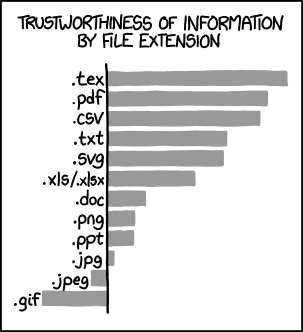
\includegraphics[scale=0.8]{file_extensions.png}
  \caption{xkcd comic.}
  \label{fig:comic}
\end{figure}
\\
\newpage
\subsection{Tables}
Tables can be a real pain to format correctly within \LaTeX{}, but are far easier within LyX, for example. Here is a table:\\

\begin{table}[htb]
\caption{An example table.}
\label{tab:tab1}
\centering
	\begin{tabular}{c|l|l}
	Pet & Size & Price [\pounds] \\ 	
	\hline
	Tree & 60m  & 500 \\
	Cat & 35cm& 60 \\
	Giant Squid & 13m & who knows \\
	Crocodile & 6m & 600 \\
	\end{tabular}
\end{table}

\noindent
We now reference one of our references \cite{LeVeque}. If using the .bib file for the bibliography you must compile first with latex, then with bibtex, then again twice with latex.

\bibliographystyle{plain}
\bibliography{Exercise_bibliography}



% This is a bibliography created within LaTeX. Note that Bibtex is the more advanced way to handle large numbers of references.
% Note the number in {} after the bibliography indicates the maximum number of references via the number of digits, eg. 56 allows for 99.

%\begin{thebibliography}{99}
%\bibitem{ref1} Person A, Person A's Paper, 
%Journal A (Date A).

%\bibitem{ref2} Person B, 
%Person B's Book, Publisher B (Date B).
 
%\end{thebibliography} 
\end{document}